\documentclass[a4paper,12pt]{article}

\usepackage[utf8]{inputenc}
\usepackage[left=0.5in,right=0.5in,top=1in,bottom=1in]{geometry}
\usepackage{amsmath,amssymb,amsfonts}
\usepackage{pgfplots,graphicx,calc,changepage}
\pgfplotsset{compat=newest}
\usepackage{enumitem}
\usepackage{fancyhdr}
\usepackage[colorlinks = true, linkcolor = blue]{hyperref}

\newcommand{\nats}{\mathbb{N}}
\newcommand{\reals}{\mathbb{R}}
\newcommand{\rats}{\mathbb{Q}}
\newcommand{\ints}{\mathbb{Z}}
\newcommand{\pols}{\mathcal{P}}
\newcommand{\cants}{\Delta\!\!\!\!\Delta}
\newcommand{\eps}{\varepsilon}
\newcommand{\st}{\backepsilon}
\newcommand{\abs}[1]{\left| #1 \right|}
\newcommand{\dom}[1]{\mathrm{dom}\left(#1\right)}
\newcommand{\for}{\text{ for }}
\newcommand{\dd}[1]{\mathrm{d}#1}
\newcommand{\spn}{\mathrm{sp}}
\newcommand{\nul}{\mathcal{N}}
\newcommand{\col}{\mathrm{col}}
\newcommand{\rank}{\mathrm{rank}}
\newcommand{\norm}[1]{\lVert #1 \rVert}
\newcommand{\inner}[1]{\left\langle #1 \right\rangle}
\newcommand{\pmat}[1]{\begin{pmatrix} #1 \end{pmatrix}}
\renewcommand{\and}{\text{ and }}

\newsavebox{\qed}
\newenvironment{proof}[2][$\square$]
    {\setlength{\parskip}{0pt}\par\textit{Proof:} #2\setlength{\parskip}{0.25cm}
        \savebox{\qed}{#1}
        \begin{adjustwidth}{\widthof{Proof:}}{}
    }
    {
        \hfill\usebox{\qed}\end{adjustwidth}
    }

\pagestyle{fancy}
\fancyhead{}
\lhead{Caleb Jacobs}
\chead{APPM 5470: PDEs}
\rhead{Homework \#1}
\cfoot{}
\setlength{\headheight}{35pt}
\setlength{\parskip}{0.25cm}
\setlength{\parindent}{0pt}

\begin{document}
\section*{Chapter 1}
\subsection*{Problem 3}
    Find an equation relating the parameters $c, m, n$ so that the function $u(x, t) = \sin(m t)\sin(n x)$ satisfies the wave equation $u_{tt} = c^2 u_{xx}$ for $ c > 0 $.
    
    First off, our derivatives are as follows,
    \begin{align*}
        u_{tt} &= -m^2 \sin(m t) \sin(n x) \\
        u_{xx} &= -n^2 \sin(m t) \sin(n x).
    \end{align*}
    Then, plugging our derivatives into the wave equation yields
    \[
        -m^2 \sin(m t) \sin(n x) = -c^2 n^2 \sin(m t) \sin(n x)
    \]
    which implies
    \[
        m^2 = c^2 n^2
    \]
    for $ c > 0 $.

\subsection*{Problem 8}
    Consider the linear transport equation (1.8) with initial and boundary conditions (1.10).
    \[
        \begin{cases}
            u_t + c u_x = 0 \\
            u(x, 0) = \phi(x), & x \geq 0 \\
            u(0, t) = \psi(t), & t \geq 0.
        \end{cases}
    \] 
    
    \begin{enumerate}[label = \textbf{(\alph*)}]
        \item Suppose the data $ \phi, \psi $ are differentiable functions. Show that the function $ u : Q_{q} \to \reals $ given by 
        \begin{equation}
            u(x, t) = \begin{cases}
                \phi(x - ct), & \text{if } x \geq ct, \\
                \psi(t - x/c), & \text{if } x \leq ct
            \end{cases}
            \label{soln:cases}
        \end{equation}
        satisfies the PDE away from the line $ x = ct $ with $c > 0$, the boundary condition, and initial conditions. 
        
        When we are away from the line, we have
        \begin{align*}
            u_t &= \begin{cases}
                -c \phi'(x - ct), & x > ct \\
                \psi'(t - x/c), & x < ct
            \end{cases} \\
            u_x &= \begin{cases}
                \phi'(x - ct), & x > ct \\
                -\frac{1}{c} \psi'(t - x/c), & x < ct
            \end{cases}.
        \end{align*}
        Using the derivatives above
        \begin{align*}
            u_t + c u_x &= \begin{cases}
                -c \phi'(x - ct) + c \phi'(x - ct), & x > ct\\
                \psi'(t - x/c) - c \frac{1}{c} \psi'(t - x/c), & x < ct
            \end{cases} \\
            &= \begin{cases}
                0, & x > ct\\
                0, & x < ct
            \end{cases} \\
            &= 0
        \end{align*}
        for $ x,t $ not on the line. So, (\ref{soln:cases})  defined above satisfies our PDE off of the line $ x = ct $. 
        
        Checking the initial condition yields
        \[
            u(x, 0) = 
            \begin{cases}
                \phi(x), & \text{if } x \geq 0, \\
                \psi(x/c), & \text{if } x \leq 0
            \end{cases} \implies
            u(x,0) = \phi(x) \text{ for } x \geq 0.
        \]
        Now, checking our boundary condition yields
        \[
            u(0, t) = 
            \begin{cases}
                \phi(- ct), & \text{if } 0 \geq ct, \\
                \psi(t), & \text{if } 0 \leq ct
            \end{cases} \implies
            u(0, t) = \psi(t) \text{ for } t \geq 0.
        \]
        So our solution solve the initial/boundary value problem.
        
        \item In solution (\ref{soln:cases}), the line $ x = ct $, which emerges from the origin $ x = t = 0 $, separates the quadrant $ Q_1 $ into two regions.
        \begin{enumerate}[label = \textbf{(\roman*)}]
            \item Find conditions on the data $ \phi, \psi $ so that the solution is continuous across the line $ x = ct $.
            
            When $ x = ct $, we have $ \phi(x - ct) = \phi(ct - ct) = \phi(0) $ and $ \psi(t - x/c) = \psi(x/c - x/c) = \psi(0)$. Thus, for continuity when $ x = ct $, we need
            \[
                \phi(0) = \psi(0).
            \]
            
            \item Find conditions on the data $ \phi, \psi $ so that the solution is differentiable across the line $ x = ct $.
            
            For differentiablity of $ u $ across the line $ x = ct $, we need differentiablity in both partial derivatives, $ u_t $ and $ u_x $ across the line. First, let's compute the derivatives on the line:
            \begin{align*}
                \left.\partial_x \phi(x - ct)\right\lvert_{x = ct}  &= \phi'(0) \\
                \left.\partial_x \psi(t - x/c)\right\lvert_{x = ct} &= -\frac{1}{c}\psi'(0) \\
                \left.\partial_t  \phi(x - ct)\right\lvert_{x = ct}  &= -c\phi'(0) \\
                \left.\partial_t  \psi(x - ct)\right\lvert_{x = ct}  &= \psi'(0).
            \end{align*}
            Equating our derivatives yields
            \begin{align*}
                \phi'(0) &= -\frac{1}{c}\psi'(0) \\
                -c\phi'(0) &= \psi'(0)
            \end{align*}
            which reduces to
            \[
                \phi'(0) = -\frac{1}{c}\psi'(0).
            \]
            So, for $ u $ to be differentiable across the line $ x = ct $, we need $ \phi'(0) = -\frac{1}{c}\psi'(0) $.
        \end{enumerate}
    \end{enumerate}

\subsection*{Problem 9}
    Let $ f : \reals \to \reals $ be differentiable. Verify that if $ u(x, t) $ is differentiable and satisfies (1.12), that is, $ u = f(x - ut) $, then $ u(x, t) $ is a solution of the initial value problem
    \[
    	u_t + u u_x = 0, \; -\infty < x < \infty, \; t > 0, \;u(x, 0) = f(x), \; -\infty < x < \infty.
    \]
    
    Suppose $ u(x,t) $ is differentiable and $ u = f(x - ut) $. Then, the initial condition is easily verified as
    \[
    	u(x,0) = f(x - u(x,0) \cdot 0) = f(x).
    \]
    Next, we can start verifying the PDE by computing the partial derivatives as follows
    \begin{align*}
        u_t  &= f'(x - u t) (-u_t t - u) \\
        u_x &= f'(x - ut) (1 - u_x t).
    \end{align*}
    Now, putting these derivative into our PDE yields
    \begin{align*}
        u_t + u u_x &= f'(x - u t) (-u_t t - u) + u f'(x - ut) (1 - u_x t) \\
        &= f'(x - ut) (-u_t t - u + u - u u_x t) \\
        &= f'(x - ut) (-u_t t - u u_x t) \\
        &= -t f'(x - ut) (u_t + u u_x).
    \end{align*}
Clearly, at $ t = 0 $ our PDE equals zero and so $ u $ satisfies the PDE at $ t = 0 $, But, when $ t > 0 $, we have
\[
    u_t + u u_x = -t f'(x - ut) (u_t + u u_x)
\]
which implies that either $ 1 = -t f'(x - ut)  $ or $ u_t + u u_x = 0 $. The first equality implies that $ f'(x - ut) = -1/t $ which doesn't hold because $ f'(x - ut) $ is differentiable everywhere but $ - 1/t $ is not differentiable at $ t = 0 $. So, we must have the second equality, $ u_t + u u_x = 0 $ which shows that $ u $ solves the IVP!

\section*{Chapter 2}
\subsection*{Problem 5}
	Find the dispersion relation $ \sigma = \sigma(\xi) $ for the following dispersive equations:
	\begin{enumerate}[label = \textbf{(\alph*)}]
		\item The beam equation $ u_{tt} = -u_{xxxx} $.
		
		Assume $ u(x,t) = e^{i\xi x + \sigma(\xi)t} $. Then,
		\begin{align*}
			u_{tt}       &= \sigma^2(\xi)u(x,t) \\
			u_{xxxx} &= \xi^4 u(x,t)
		\end{align*}
		which implies
		\begin{align*}
			& \sigma^2(\xi)u(x,t) = -\xi^4 u(x,t) \\
			\implies & \sigma^2(\xi) = -\xi^4 \\
			\implies & \sigma(\xi) = \pm i \xi^2.
		\end{align*}
		From the dispersion relation $ \sigma(\xi) = \pm i \xi^2 $, we can see that $ u(x,t) $ is not dissipative because $ \sigma(\xi) $ is purely imaginary and thus each Fourier term in the solution will not decay with a change in time. However, $ u(x,t) $ is dispersive because 
		\[
			u(x,t) = e^{i \xi x \pm i \xi^2 t} = e^{i \xi (x \pm \xi t)}
		\]
		which shows that the wave speed $ \pm \xi $ is dependent on the wave number $ \xi $. In the case of the wave equation, the wave speed is invariant with respect to the wave number and so the wave equation is not dispersive.
		
		\item The linear Benjamin-Bona-Mahoney (BBM) equation $ u_t + c u_x + \beta u_{xxt} = 0 $.
		
		Similar to before, assume $ u(x,t) = e^{i\xi x + \sigma(\xi)t} $. Then
		\begin{align*}
			u_t        &= \sigma(\xi) u(x,t) \\
			u_x       &= i \xi u(x,t) \\
			u_{xxt} &= -\xi^2 \sigma(\xi) u(x,t)
		\end{align*}
		which implies
		\begin{align*}
			& \sigma(\xi)u(x,t) + i \xi c u(x,t) - \xi^2\beta \sigma(\xi) u(x,t) = 0 \\
			\implies & \sigma(\xi) + i \xi c - \xi^2\beta \sigma(\xi) = 0 \\
			\implies & \sigma(\xi)(1 - \xi^2 \beta) = -i c \xi \\
			\implies & \sigma(\xi) = \frac{i c \xi}{\xi^2 \beta - 1}.
		\end{align*}
		Just like part \textbf{(a)} our dispersion relation $ \sigma(\xi) = \frac{i c \xi}{\xi^2 \beta - 1} $ is purely imaginary and so our solution is a traveling wave without dissipation. Furthermore,
		\[
			u(x,t) = e^{i \xi x + \frac{i c \xi}{\xi^2 \beta - 1} t} = e^{i \xi \left (x -\left (- \frac{c}{\xi^2 \beta - 1}\right ) t\right )}
		\]
		shows that the wave speed is given by $ -\frac{c}{\xi^2 \beta - 1} $ which changes depending on the wave number. Thus, because the speed is dependent on the wave number, our solution is dispersive in time. A large difference between the wave speed of the KdV $ c - \beta \xi^2 $ and the wave speed of the BBM is that the wave speed of the KdV is unbounded with respect to the wave number while the speed of the BBM is bounded.
	\end{enumerate}

\subsection*{Problem 6}
	Suppose in the traffic flow model discussed in Section 2.4 that the speed $ v $ of cars is taken to be a positive monotonic differentiable function of density: $ v = v(u) $
	\begin{enumerate}[label = \textbf{(\alph*)}]
		\item Should $ v $ be increasing or decreasing?
		
		In a traffic flow model, we should have $ v $ decreasing as density $ u $ increases. As cars get backed up ($ u $ increases), the speed at which cars can navigate through traffic would go down ($ v $ decreases).
		
		\item How would you characterize the maximum velocity $ v_\text{max} $ and the maximum density $ u_\text{max} $?
		
		Maximum speed should occur when the density of the cars is minimized (i.e. $ v_{\text{max}} = v(0) $). On the other hand, we should have maximum density of cars when the speed is minimized (i.e. $ v(u_\text{max}) = 0 $).
		
		\item Let $ Q(u) = u v(u) $. Prove that $ Q $ has a maximum at some density $ u^* \in (0,u_\text{max})$.
		
		First, we know $ v $ is continuous on $ [0, u_\text{max}] $ and so $ Q(u) = u v(u) $ is continuous on $ [0, u_\text{max}] $. So, by the Extreme Value Theorem, there exists a point $ u^* \in [0,u_\text{max}] $ such that $ Q(u^*) $ is a maximum on $ [0, u_\text{max}] $. Then, note that 
		\[
			Q(0) = 0 v(0) = 0
		\]
		and
		\[
			Q(u_\text{max})  = u_\text{max} v(u_\text{max}) = u_\text{max} 0 = 0.
		\]
		 But, $ v(u) > 0$ for $ u \in (0, u_\text{max}) $ and so is $ u $, therefore $ Q(u) > 0 $ for $ u \in (0, u_\text{max}) $. Thus, because $ Q(u) > 0 $ for $u \in (0, u_\text{max})$, $ Q(0) = 0 $, and $ Q(u_\text{max}) = 0 $, we can restrict the domain of $ u^* $ to $ u^* \in (0, u_\text{max}) $. Therefore, $ Q $ contains a maximum at $u^* \in (0, u_\text{max})$.
		
		\item Can there be two local maxima of the flux?
        
        There can be two local maxima of the flux. Consider $ v(u) = -(u - 2)^3 + 1 $ which is a positive monotonic function. Using this $ v(u) $, yields a $ Q(u) = u*v(u) =  -u(u - 2)^3 + 1 $. Plotting our $ Q(u) $ from $ u = 0 $ to $ u = u_\text{max} $ produces
        
        \begin{figure*}[h!]
            \centering
            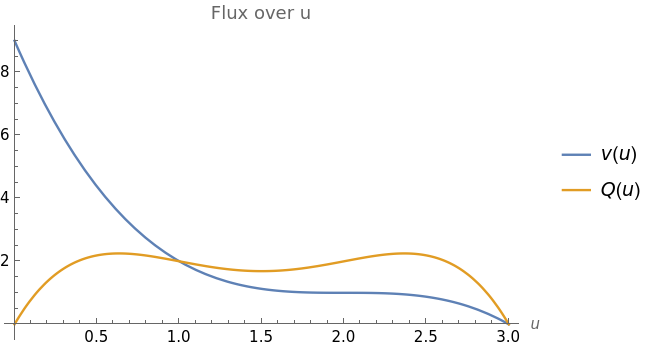
\includegraphics[width = 0.5\textwidth]{images/two_humps.png}
        \end{figure*}
    
        From the figure, we can clearly see two local maxima of the flux which work to be at $ u = \frac{3 - \sqrt{3}}{2} $ and $ u = \frac{3 + \sqrt{3}}{2} $ respectively.
	\end{enumerate}

\section*{Additional Problems}
\subsection*{Problem A1}
    Consider the initial/boundary value problem for the transport equation
    \[
        \left\{\begin{array}{lll}
            u_t + u_x = 0, & t > 0, & x > bt \\
            u(bt, t) = f(t), & t > 0 \\
            u(x,0) = g(x), & x > 0
        \end{array}\right.
    \]
    where $ \abs{b} < 1$ is the velocity of a source emitting the time-varying signal $ f(t) $, and $ f, g \in C^1(0, \infty) $.
    \begin{enumerate}[label = \textbf{(\alph*)}]
        \item Solve the initial/boundary value problem when $ g(x) = 0 $ and $ f(t) $ may be any $ C^1 $ function such that $ \lim_{t \to 0^+} f(t) = 0 $.
        
        To begin solving this initial/boundary value problem, notice that the PDE can be solved using the Method of Characteristic where we have two smooth surfaces of Cauchy data. We will call our initial condition $ \Gamma_1 $ and our boundary condition $ \Gamma_2 $. Let's parameterize our conditions as
        \[
            \begin{array}{rl}
                \Gamma_1: & \vec{r}(s) = \langle x_0(s), t_0(s), z_0(s) \rangle = \langle s, 0, g(s)  \rangle \\
                \Gamma_2: & \vec{r}(s) = \langle x_0(s), t_0(s), z_0(s) \rangle = \langle bs, s, f(s)  \rangle \\
            \end{array}
        \]
        where $ s > 0 $. Next, we can extract the system of ODEs that depend on our temporary variable $ \tau $ as
        \[
            \frac{\partial x}{\partial \tau} = 1, \qquad \frac{\partial t}{\partial \tau} = 1, \qquad \frac{\partial z}{\partial \tau} = 0.
        \]
        Now that we have our ODEs and the Cauchy data parameterized, we can solve for our characteristic solutions off of each surface. We will start by solving off of $ \Gamma_1 $ by assuming $ s $ is fixed which leads to
        \[
            \begin{array}{rccl}
                \frac{\partial x}{\partial \tau} = 1, & x(0) = x_0(s) = s & \implies & x(\tau, s) = \tau + s \\
                \frac{\partial t}{\partial \tau} = 1, & t(0) = t_0(s) = 0 & \implies & t(\tau, s) = \tau \\
                \frac{\partial z}{\partial \tau} = 0, & z(0) = z_0(s) = g(s) & \implies & z(\tau, s) = g(s)
            \end{array}
        \]
        Next, we will invert our solution so we have $ \tau(x,t) $ and $ s(x,t) $  by solving the simple linear system above as
        \begin{align*}
            \tau(x,t) &= t \\
            s(x,t) &= x - t.
        \end{align*}
        using these characteristics, we can write our solution originating from $ \Gamma_1 $ as
        \begin{equation}
            u(x,t) = z(\tau(x,t), s(x,t)) = g(x - t). \label{soln:gamma1}
        \end{equation}
    
        Now, we can solve for the solution off of $ \Gamma_2 $ by combining the parameterization of $ \Gamma_2 $ and the system of ODEs to get
        \[
            \begin{array}{rccl}
                \frac{\partial x}{\partial \tau} = 1, & x(0) = x_0(s) = bs & \implies & x(\tau, s) = \tau + bs \\
                \frac{\partial t}{\partial \tau} = 1, & t(0) = t_0(s) = s & \implies & t(\tau, s) = \tau + s\\
                \frac{\partial z}{\partial \tau} = 0, & z(0) = z_0(s) = f(s) & \implies & z(\tau, s) = f(s).
            \end{array}
        \]
        Just like last time, we can invert this linear system to find our characteristics as
        \begin{align*}
            \tau(x,t) &= t - \frac{x - t}{b - 1} \\
            s(x,t) &= \frac{x - t}{b - 1}.
        \end{align*}
        Finally, we can write our solution originating from $ \Gamma_2 $ as
        \begin{equation}
            u(x,t) = z(\tau(x,t), s(x,t)) = f(\frac{x - t}{b - 1}). \label{soln:gamma2}
        \end{equation}
    
        So now we have two partial solutions that can combine to make the complete solution. To combine solutions (\ref{soln:gamma1}) and (\ref{soln:gamma2}), we need to find in what regions they are valid. If we look at each solution, we can see that the characteristics each satisfy
        \[
            x - t = c
        \]
        where $ c \in \reals $ is a constant. Each surface touches at the origin which marks the spot that the two solutions meet. So, the characteristic originating from the origin is
        \[
            x - t = 0 \implies x = t
        \]
        which is our boundary line between the two solutions where (\ref{soln:gamma1}) fills the solution space when $ x > t $ and (\ref{soln:gamma2}) fills the solution space when $ x < t $. Looking back at the original differential equation, we can see that we have $ x > bt $ for $ \abs{b} < 1 $ which further restricts the (\ref{soln:gamma2}) to $ bt < x < t $. So, our full solution is
        \begin{equation}
            u(x,t) = 
                \begin{cases}
                    g(x - t), & x > t \\
                    f(\frac{x - t}{b - 1}), & bt < x < t
                \end{cases}. \label{soln:full}
        \end{equation}
    
        Using the full solution, we can obtain a solution when $ g(x) = 0 $ as
        \[
            u(x,t) = 
            \begin{cases}
                0 & x > t \\
                f(\frac{x - t}{b - 1}), & bt < x < t
            \end{cases}.
        \]
        
        \item Now suppose the source emits the time-periodic signal $ f(t) = \sin(\omega t) $ with frequency $ \omega > 0 $. For what values of the velocity $ b $ is the frequency ``heard'' by a receiver situated at $ x = 10 $ higher than $ \omega $? When is the received frequency lower? Explain the Doppler effect.
        
        To understand how the velocity affects the perceived frequency, when a source is moving towards the receiver, the frequency generated by the source is getting ``squished'' towards the receiver. The effect is that the frequency will increase from the perspective of the receiver. If the source was moving away from the receiver, then the perceived frequency would be lower than the actual source frequency. This phenomena is known as the Doppler Effect.
        
        In the context of this PDE, if a receiver was placed at $ x = 10 $, the perceived frequency would be higher than $ \omega $ when $ b > 0 $. On the other hand, when $ b < 0 $, the perceived frequency will be lower than $ \omega $.
        
        \item Solve the initial/boundary value problem when $ f(t) = 0 $.
        
        Using solution (\ref{soln:full}) with $ f(t) = 0 $ yields the solution
        \[
            u(x,t) = 
            \begin{cases}
                g(x - t), & x > t \\
                0, & bt < x < t
            \end{cases}.
        \]
        
        \item Solve the full initial/boundary value problem.
        
        Again, using (\ref{soln:full}) with general functions $ f,g \in C^1(0, \infty) $ yields the full solution
        \[
            u(x,t) = 
                \begin{cases}
                    g(x - t), & x > t \\
                    f(\frac{x - t}{b - 1}), & bt < x < t
                \end{cases}.
        \]
        
        \item What happens if $ b \geq 1 $?
        
        To understand what happens when $ b \geq 1 $, we need to note that the transport equation above transports waves at a constant speed of 1 unit in the $ +x $ direction per one unit of time $ t $. Thus, when $ b \geq 1$, the velocity of the source is moving as fast or faster than the speed of wave transportation (i.e. faster than the speed of sound). As a result, the frequency generated by the source will start to intersect with the characteristics originating from the initial  condition. In other words, there will be a shock from the clashing characteristics. We would need to do a bit more work on the PDE to obtain a more well defined solution for when $ b \geq 1 $.
    \end{enumerate}

\subsection*{Problem A2}
    Classification of linear, second order PDEs:
     \begin{enumerate}[label = \textbf{(\alph*)}]
            \item Determine the type of the equation $ u_t = u_{xx} + 2 u_x + u $.
            
            To determine the type of the PDE, we can write out the coefficient matrix $ A $ of the highest degree derivative terms as 
            \[
                A =
                \pmat{
                    1 & 0 \\
                    0 & 0
                }.
            \]
            Next, we can compute the eigenvalues as $ \lambda \in \{1, 0\} $. We have one non-zero eigenvalue and one zero eigenvalue which tells us that $ u_t = u_{xx} + 2 u_x + u $ is a parabolic PDE.
            
            \item Determine the type of the equation $ u_{tt} + 2 \alpha u_{xt} + u_{xx} = 0 $ for each value of the parameter $ \alpha $.
            
            Similar to part \textbf{(a)}, we will start by forming the coefficient matrix of the highest degree derivatives as
            \[
                A =
                \pmat{
                    1 & \alpha \\
                    \alpha & 1
                }.
            \]
            Now, we can compute the eigenvalues of $ A $ to get the two eigenvalues $ \lambda \in \{1 + \alpha, 1 - \alpha\} $. Thus, we can get two positive eigenvalues if $ \abs{\alpha} < 1 $ which makes the PDE elliptic. Furthermore, we can get two opposite sign eigenvalues if $ \abs{\alpha} > 1 $ which would make the PDE hyperbolic. Lastly, we can get one zero eigenvalue and one non-zero eigenvalue if $ \abs{\alpha} = 1 $ which would make the PDE parabolic. In summary, $ u_{tt} + 2 \alpha u_{xt} + u_{xx} = 0 $ will have the following types
            \[
                \text{(Second Order PDE Type)} =
                \begin{cases}
                    \text{Elliptic}, & \abs{\alpha} < 1 \\
                    \text{Parabolic}, & \abs{\alpha} = 1 \\
                    \text{Hyperbolic}, & \abs{\alpha} > 1
                \end{cases}.
           \] 
            
            \item For the equation in part \textbf{(b)}, what values of $ \alpha $ ensure solutions of the form $ u(x,t) = f(x - ct) $ with $ c \in \reals $, provided $ f(x) $ is twice differentiable. For what values of $ \alpha $ is $ u(x,t) = t f(x - ct) $ a solution? What values does $ c $ take in this case?
            
            To find criteria on $ \alpha $ to make $ u(x,t) = f(x - ct) $ a solution to our PDE, let's first compute the needed derivatives for the PDE as
            \begin{align*}
                u_{tt} &= c^2 f''(x - ct) \\
                u_{xt} &= -c f''(x - ct) \\
                u_{xx} &= f''(x - ct). 
            \end{align*}
            Now, plugging these derivatives into the PDE yields
            \begin{align*}
                & c^2 f''(x - ct) - 2 \alpha c f''(x - ct) + f''(x - ct) = 0 \\
                \implies & c^2 - 2 \alpha c + 1 = 0 \\
                \implies & \alpha = \frac{c^2 + 1}{2c}
            \end{align*}
            provided $ c \neq 0 $. If $ c = 0 $, then we can have any $ \alpha \in \reals $.
            
            Now, let's find criteria on $ \alpha $ and $ c $ to make $ u(x,t) = t f(x - ct) $ a solution. Just like the first part, let's compute our needed derivatives as
            \begin{align*}
                u_{tt} &= c^2 t f''(x - ct) - 2c f'(x - ct) \\
                u_{xt} &= f'(x - ct) - c t f''(x - ct) \\
                u_{xx} &= t f''(x - ct). 
            \end{align*}
            To find our criteria, we can plug these derivatives into the PDE and factor out anything in common to get
            \[
                (c^2 - 2 \alpha c + 1) t f''(x - ct) + 2(\alpha - c) f'(x - ct) = 0.
            \]
            Then, because $ t f''(x - ct) $ and $ f'(x - ct) $ are not necessarily constant as $ x $ and $ t $ change, we must have the system of equations
            \begin{align*}
                c^2 - 2 \alpha c + 1 &= 0 \\
                2(\alpha - c) &= 0
            \end{align*}
            which yields
            \[
                \alpha = c
            \]
            and finally two solutions of ($ \alpha = 1 $ and $ c = 1 $) or ($ \alpha = -1 $ and $ c = -1 $).
            
            \item Classify the equation $ xyu_{xx} + 4u_{xy} - (x^2 + y^2)u_{yy} - u = 0 $ throughout the $ (x,y) $-plane.
            
            Just as in part \textbf{(a)} and \textbf{(b)}, we will construct the coefficient matrix to our PDE as
            \[
                A =
                \pmat{
                    xy & 2 \\
                    2 & -(x^2 + y^2)
                }
            \]
            which has two eigenvalues
            \begin{align*}
                \lambda_1 &= \frac{1}{2} \left(-x^2 + x y - y^2 -  \sqrt{x^4+2 x^3 y+3 x^2 y^2+2 x y^3+y^4+16}\right), \\
                \lambda_2 &= \frac{1}{2} \left(-x^2 + x y - y^2 + \sqrt{x^4+2 x^3 y+3 x^2 y^2+2 x y^3+y^4+16}\right)
            \end{align*}
            which simplify to
            \begin{align*}
                \lambda_1 &= \frac{1}{2} \left(-x^2 + x y - y^2 - \sqrt{\left(x^2+x y+y^2\right)^2+16} \right), \\
                \lambda_2 &= \frac{1}{2} \left(-x^2 + x y - y^2 + \sqrt{\left(x^2+x y+y^2\right)^2+16} \right).
            \end{align*}
            Now, to understand the different types of PDEs we have depending our place in the $ (x,y) $-plane, we will check the sign of $ \lambda_1 $. Consider
            \begin{align*}
                -x^2 + xy - y^2 &< x^2 + xy + y^2 \\
                &\leq \sqrt{(x^2 + xy + y^2)^2} \\
                &< \sqrt{16 + (x^2 + xy + y^2)^2}.
            \end{align*}
            Next, we can rearrange our inequality to get
            \[
                -x^2 + xy - y^2 - \sqrt{16 + (x^2 + xy + y^2)^2} < 0
            \]
            or in other words
            \[
                \lambda_1 < 0
            \]
            for all $ x,y \in \reals $. So, now that we know $ \lambda_1 $ is purely negative, it is up to $ \lambda_2 $ to set the type of second order PDE. 
            
            Let's find an expression for the roots or boundaries of $ \lambda_2 $. Consider $ \lambda_2 = 0 $ which becomes
            \begin{align*}
                & \frac{1}{2} \left(-x^2 + x y - y^2 + \sqrt{\left(x^2+x y+y^2\right)^2+16} \right) = 0 \\
                \implies & -x^2 + x y - y^2 = \sqrt{\left(x^2+x y+y^2\right)^2+16} \\
                \implies & \left(-x^2 + x y - y^2 \right)^2 = \left(x^2+x y+y^2\right)^2 +16 \\
                \implies & \left(-x^2 + x y - y^2 \right)^2 - \left(x^2+x y+y^2\right)^2 = 16 \\
                \implies & \left(-x^2 + x y - y^2 + x^2+x y+y^2\right)\left(-x^2 + x y - y^2 - x^2 - x y - y^2\right) = 16\\
                \implies & \left(2x y\right)\left(-2x^2 - 2y^2\right) = 16 \\
                \implies & x y\left(x^2 + y^2\right) = -4.
            \end{align*}
            Thus, our boundary PDEs (parabolic PDEs) will take place anytime $ x y\left(x^2 + y^2\right) = -4 $. Furthermore, when $ \lambda_2 > 0 $, we will have hyperbolic PDEs which takes place in the region that contains the origin. The two regions not containing the origin satisfy $ \lambda_2 < 0 $ contain the elliptic PDEs. The figure below illustrates the different regions and boundary regions
            \begin{figure}[h!]
                \centering
                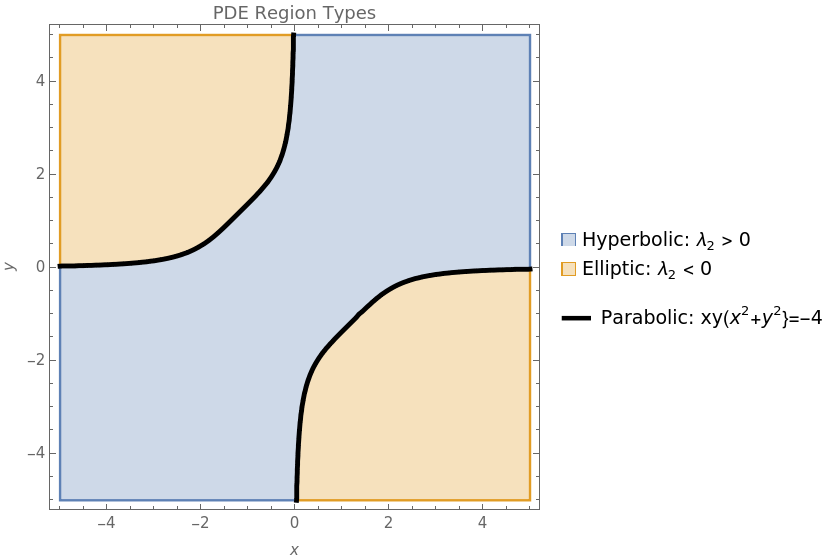
\includegraphics[width = 0.5\textwidth]{images/PDE_Types.png}
            \end{figure}
     \end{enumerate}
\end{document}